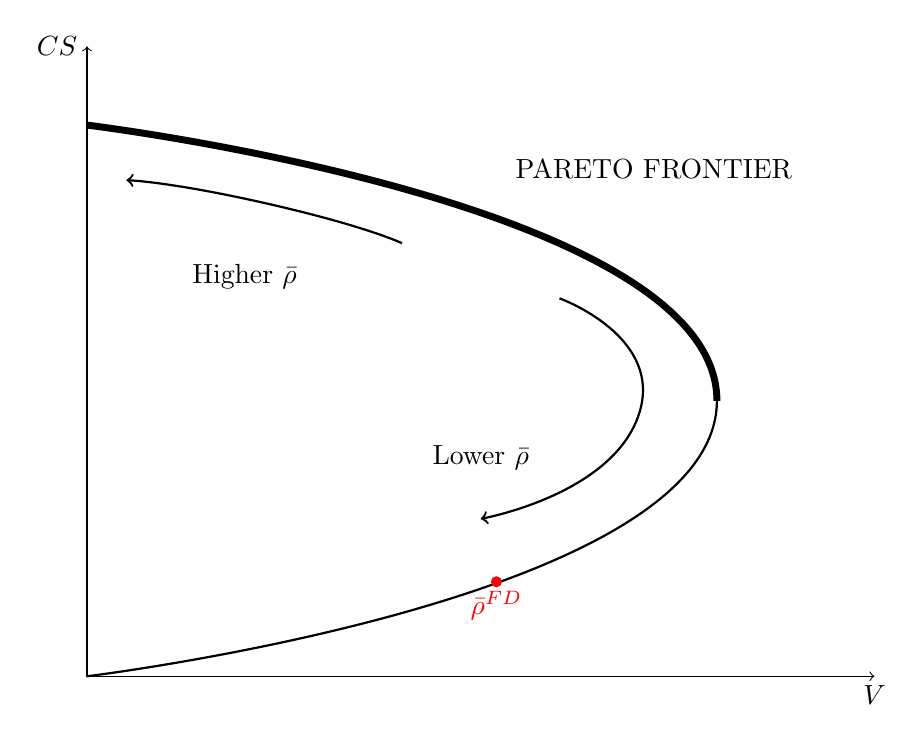
\begin{tikzpicture}[xscale=1,yscale=1] 

		\draw [<->] (0,8) node (yaxis)[left] {$CS$} 
		        |- (10,0) node (xaxis) [below] {$V$};
	\def\mycoordinates{(0,0) (8,3.5) (0,7)}

	%\draw[step=1cm,gray,very thin] (0,0) grid (10,8);

	\def\mycoordinates{(0,0) (8,3.5) (0,7)}

	\draw[thick] plot [smooth,tension=1.3] coordinates {\mycoordinates};
	\begin{scope}
	    \clip (0,3.5) rectangle (10,8);
	    \draw [line width=2.5] plot [smooth,tension=1.3] coordinates {\mycoordinates};
	  \end{scope}

        %\fill (0,0)  circle (2pt) ;
	%\node at (.9,.2)[above] {$\bar\rho=0$};
%      \fill (8,3.5)  circle (2pt) ;
%	\node at (8,3.7)[right] {$\alpha^{coord}$};
       % \fill (0,7)  circle (2pt) ;
	%\node at (0,7.5)[right] {$\bar\rho^{max}\leq 1$};
	

	%\draw[thick] plot [smooth,tension=1.3] coordinates {\mycoordinates};

%	\draw [->,thick] (4,5.5) to  (.5,6.3);
	\draw[thick,->] plot [smooth,tension=1.3] coordinates {(4,5.5)  (2.3,6) (.5,6.3)};

	\draw[thick,->] plot [smooth,tension=1.3] coordinates {(6,4.8) (7,3.3) (5,2)};

%	\draw [->,thick] (6,4.5) to  [out=-30,in=30] (5,2);


	\node at (7.2,6.2) [above] {PARETO FRONTIER};


	\node at (2,4.8) [above] {Higher $\bar\rho$};

	\node at (5,2.5) [above] {Lower $\bar\rho$};


	\coordinate (A) at (5.2,1.2);
        \fill[red] (A)  circle (2pt) ;
	\node at (A) [below,red] {$\bar\rho^{FD}$};




        
\end{tikzpicture}